\chapter{Cryptography}

Cryptography is a powerful tool that enables secure communication over insecure communication channels. It forms the basis for many security mechanisms, e.g. online browsing. It is not a solution to all security problems, but it is reliable if implemented and used properly.

Cryptography provides mechanisms to achieve these goals:

1. \textbf{Confidentiality}: preventing adversaries from learning the content of our private data

2. \textbf{Integrity}: preventing adversaries from altering our data

3. \textbf{Authenticity}: ensuring the data is created by the expected user

\section{Basic Concepts}

\subsection{Terminologies}
1. \textbf{Encryption}: converting plaintext into ciphertext

2. \textbf{Decryption}: converting ciphertext into plaintext

3. \textbf{Key}: a randomly chosen value used in encryption and decryption

4. \textbf{Cryptanalysis}: breaking the encryption/decryption scheme by analyzing the algorithm or implementation

\subsection{Types of Cryptographic Algorithms}
1. \textbf{Symmetric Algorithms}: use a single shared secret key

2. \textbf{Asymmetric Algorithms}: use a pair of keys (public/private). It is computationally impractical to derive one key from the other.

\subsection{Cryptographic Functions}
A \textbf{one-way function} is easy to compute but difficult to invert.

A \textbf{cryptographic hash function} produces a fixed-length output and satisfies:

- pre-image resistance

- second pre-image resistance

- collision resistance

Cryptographic algorithms can be computationally secure, since the cost of breaking the cipher is unacceptably high and the time required to break it exceeds the useful lifetime of the encrypted information.

\section{Threat Model, Attacks and Security}

\subsection{Threat Model and Attacks}

Before constructing secure systems, we define attacker capabilities:

1. \textbf{Ciphertext-Only Attack (COA)}: attacker sees ciphertexts only

2. \textbf{Known Plaintext Attack (KPA)}: attacker knows some plaintext-ciphertext pairs

3. \textbf{Chosen Plaintext Attack (CPA)}: attacker can choose plaintexts to be encrypted

4. \textbf{Chosen Ciphertext Attack (CCA)}: attacker can choose ciphertexts to be decrypted

A secure scheme must remain secure even under strong attack models (e.g. CPA).

\subsection{Security Definitions}

\subsubsection{Pseudo-Random Permutation (PRP)}
Encryption should behave like a random permutation to any efficient attacker.

\begin{intuition}
  The attacker can query inputs and observe the outputs from two boxes, one implementing \(E_K\) and one implementing a random permutation. Although the same input always produces the same output, the attacker cannot find any pattern to distinguish which box is the real encryption. Hence, the cipher behaves like a random shuffling, achieving PRP security.
\end{intuition}

We say an encryption scheme is PRP secure if for any polynomial-time attacker, the probability of winning this security game is not significantly greater than \(50\%\), i.e.,
\[
  \mathbb{P}[\text{Attacker wins}] \leq \frac{1}{2} + \varepsilon \quad (\text{e.g., } \varepsilon = \frac{1}{2^{128}})
\]
However, the attacker may still learn whether two plaintexts are equal, since \(E_K(M_i) = E_K(M_j)\) implies \(M_i = M_j\), even though the actual values of \(M_i\) and \(M_j\) remain unknown.

\subsubsection{Indistinguishability under Known Plaintext Attack (IND-KPA)}
Even with known plaintexts, attacker cannot distinguish encryptions.

\begin{intuition}
  The attacker has access to some plaintext--ciphertext pairs from previous observations. Even with this knowledge, they should not be able to gain any additional information about new ciphertexts or recover the underlying plaintexts. Thus, past knowledge does not help the attacker break the encryption, which corresponds to IND-KPA security.
\end{intuition}

An encryption scheme is IND-KPA secure if and only if, for any polynomial-time attacker, the probability of winning the IND-KPA game is not significantly greater than \(50\%\), i.e.,
\[
  \mathbb{P}[\text{Attacker wins}] \leq \frac{1}{2} + \varepsilon \quad (\text{e.g., } \varepsilon = \frac{1}{2^{128}})
\]

\subsubsection{Indistinguishability under Chosen Plaintext Attack (IND-CPA)}
Even if attacker can choose plaintexts, they cannot distinguish which message was encrypted.

\begin{intuition}
  The attacker can choose arbitrary plaintexts and obtain their corresponding ciphertexts. Despite this strong capability, when given a ciphertext of one of two chosen messages, the attacker still cannot determine which message was encrypted with probability better than random guessing. This means the encryption reveals no useful information even under active attack, achieving IND-CPA security.
\end{intuition}

An encryption scheme is IND-CPA secure if and only if, for any polynomial-time attacker, the probability of winning the IND-CPA game is not significantly greater than \(50\%\), i.e.,
\[
  \mathbb{P}[\text{Attacker wins}] \leq \frac{1}{2} + \varepsilon \quad (\text{e.g., } \varepsilon = \frac{1}{2^{128}})
\]

\textbf{Key insight:} IND-CPA requires \textbf{randomized encryption}, so for the same plaintext it outputs a different ciphertext each time.

\section{Symmetric Key Cryptography}

In symmetric key encryption, a random nonce\footnote{A cryptographic nonce is an arbitrary, unique number employed in cryptographic protocols to ensure communication freshness and security.} is sometimes used in the cipher.

\subsection{Basic Model}
Let message \(M\), key \(K\), ciphertext \(C\):
\[
  C = E_K(M), \quad M = D_K(C)
\]
Here, the goal is first to ensure confidentiality. There are three algorithms involved:

1. \(\texttt{KeyGen()} \to K\)

2. \(E(M, K) = E_K(M) = C\)

3. \(D(C, K) = D_K(C) = M\)

Correctness requires:
\[
  D_K(E_K(M)) = M
\]
Note that ciphertext should reveal \textbf{no information} about plaintext (except length).

A secure scheme ensures:
\[
\mathbb{P}(\text{guessing any bit correctly}) = 0.5
\]
Any advantage \(> 0.5\) implies information leakage.

\begin{remark}
  The `slightly better than \(50\%\)' matters because, for a secure encryption scheme, every bit should appear random. Thus, an attacker guessing a bit should have
  \[
    \mathbb{P}(\text{correct}) = 0.5.
  \]
  If the probability is greater than \(0.5\), the encryption leaks information.
\end{remark}

\subsection{Simple Cipher}
A simple cipher is the Caesar cipher, e.g.
\[
  E(M,K) = M + K \mod 26
\]

This cipher is insecure due to:

- brute force

- frequency analysis

- CPA/KPA attacks

According to \textbf{Kerckhoffs's Principle}, \textit{security must rely only on secrecy of the key}. It is not sufficient to say that an attacker cannot decrypt the ciphertext; such a system should still be considered insecure. 

\subsection{One-Time Pad (OTP)}
A random key is chosen for each message \(M\), and the key is used only once. The key is as long as the message. Then we use \(E(M, K) = M \oplus K\) and \(D(C, K) = C \oplus K = (M \oplus K) \oplus K = M\).

OTP is secure against one-time eavesdropping, and the ciphertext reveals no information about the plaintext except for the length.

To prove OTP is IND-KPA secure, we assume the adversary knows some pairs \((M_0, C_0), (M_1, C_1), \dots\). Since each encryption uses a fresh independent key, there is no relation between the old and new pairs. So for any \(M_0, M_1\),
\[
  \mathbb{P} (C^* \mid M_0) = \mathbb{P} (C^* \mid M_1)
\]
so
\[
  \mathbb{P} (M_0 \mid C^*) = \mathbb{P} (M_1 \mid C^*)
\]

To prove it is IND-CPA secure, since the attacker can query \(E(M_0)\), \(E(M_1)\), we obtain a challenge ciphertext \(C^* = E(M_b)\). For each encryption, a new random key is used, so the ciphertext looks completely random every time, giving \(\mathbb{P}(\text{correct}) = \frac{1}{2}\).

However, there are several problems regarding the one-time pad.

1. Key Generation: it needs truly random and independent keys.

2. Key Distribution: it needs a secure way to distribute the random key for each communication; however, if the key can already be shared securely, such a method could be used directly to send the secret message.

3. Key Length: the key needs to be as long as the message.

\section{More on Symmetric Key Cryptography}

\subsection{Block Cipher}
Consider the building blocks as follows:

1. A function \(E: \{0, 1\}^n \times \{0, 1\}^k \to \{0, 1\}^n\)

2. Fixing the key \(K\): \(E_K: \{0, 1\}^n \to \{0, 1\}^n\)

3. Encryption \(E_K(M) = E(M, K)\)

with the following properties:

1. Correctness: \(E_K\) is a permutation (bijective)

2. Efficiency: Computation is very fast

3. Security: the permutation looks random without knowing \(K\)

For an unknown key, \(E_K\) behaves like a random permutation (PR). The attacker then cannot learn the plaintext given only the ciphertext, and thus block ciphers provide some confidentiality. However, with the same key, a block cipher produces the same output for the same input; thus, this deterministic behavior makes it not IND-CPA secure.

\subsection{Modes of Operation}
To ensure that we can encrypt messages of arbitrary lengths and achieve IND-CPA security even if the same key is reused, we apply different modes of operation.

Similar to OTP, a block cipher works on fixed-length input. If the message is shorter than the block length, padding can be added. If the message is longer, the block cipher can be applied repeatedly. This is called a block cipher mode, a rule for how to use a block cipher to encrypt long messages securely.

Chaining block ciphers in certain modes of operation invokes the block cipher multiple times on inputs related to other blocks. This requires some initial randomness, i.e. an Initialization Vector (IV). This prevents the encryption scheme from being deterministic.

\subsection{Electronic Code Book (ECB) Mode}
This is the simplest mode. It splits a long message into \(n\)-bit blocks \(M_1, M_2, \dots\). Each block is encrypted or decrypted independently using the same key, i.e. \(C_i = E_K (M_i), M_i = D_K (C_i)\). The output is produced by concatenating the encrypted or decrypted blocks (Figure 3.1).

However, this mode is insecure because it leaks patterns (Figure 3.2).

\begin{minipage}{0.5\textwidth}
\begin{figure}[H]
  \centering
  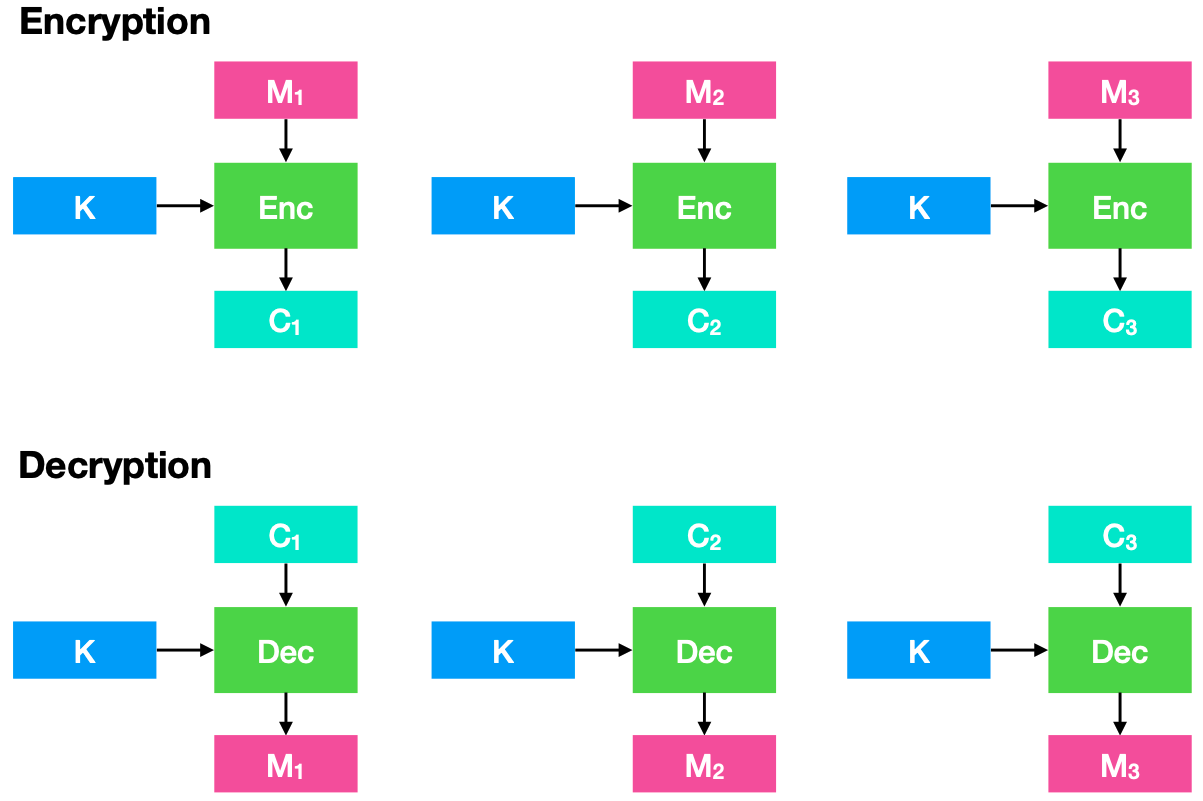
\includegraphics[width=0.7\textwidth]{Figure/ECB.png}
  \caption{ECB Mode}
\end{figure}
\end{minipage}
\begin{minipage}{0.5\textwidth}
\begin{figure}[H]
  \centering
  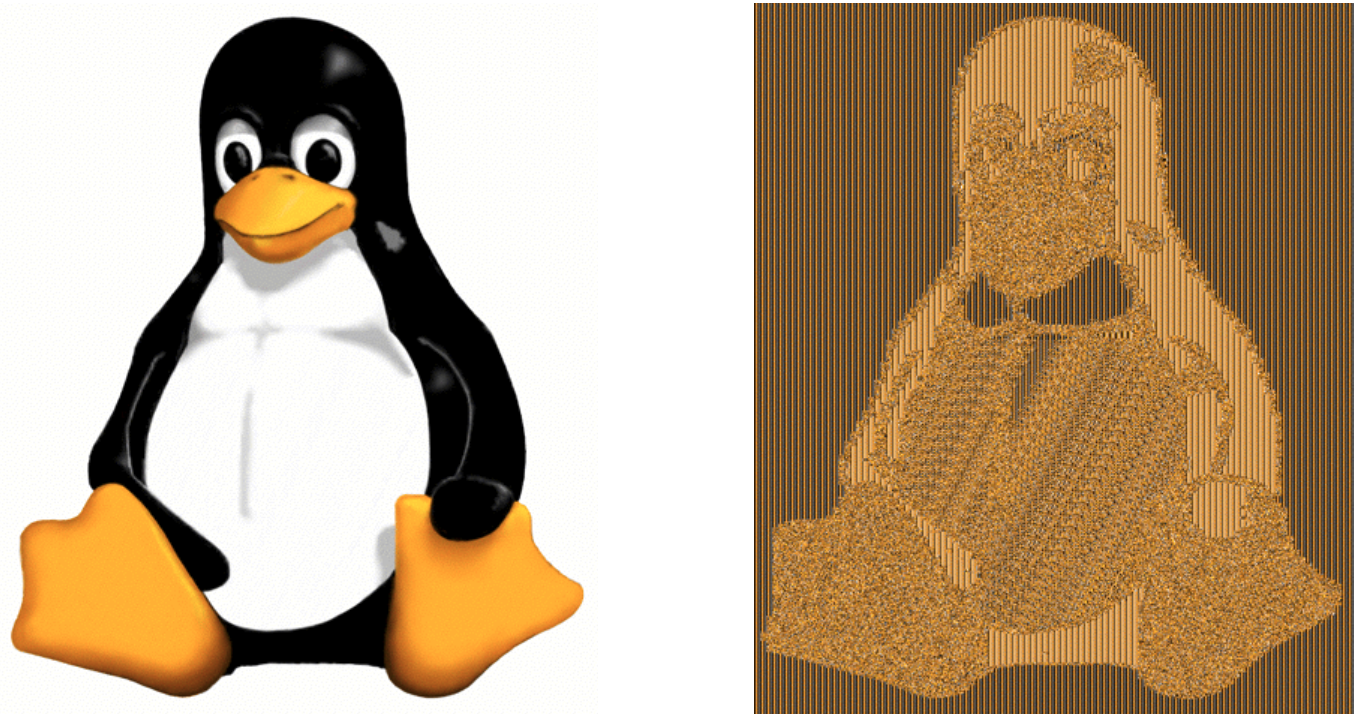
\includegraphics[width=0.7\textwidth]{Figure/ECB_Linux.png}
  \caption{Encrypted Image by ECB Mode}
\end{figure}
\end{minipage}

\subsection{Cipher Block Chaining (CBC) Mode}
A better mode is to include a varying and known nonce. Again, a long message is split into blocks. Then a one-time random IV is chosen, and the block ciphers are chained by including the output of the previous block as input to the current block. The final output is the IV concatenated with all ciphertext blocks (Figure 3.3).

This can achieve IND-CPA security, and thus it is popular and still widely used. However, it uses sequential encryption and is hard to parallelize.

\begin{minipage}{0.5\textwidth}
\begin{figure}[H]
  \centering
  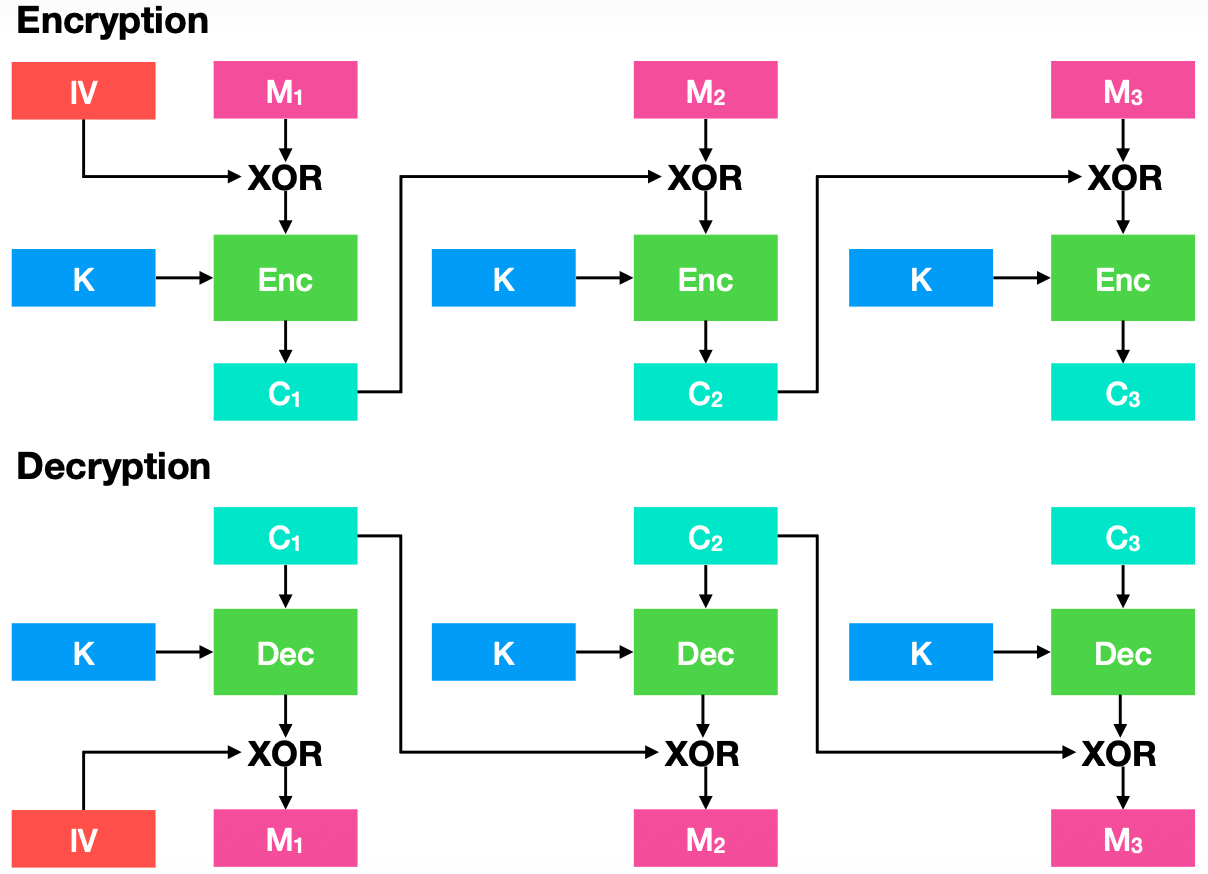
\includegraphics[width=0.7\textwidth]{Figure/CBC.png}
  \caption{CBC Mode}
\end{figure}
\end{minipage}
\begin{minipage}{0.5\textwidth}
\begin{figure}[H]
  \centering
  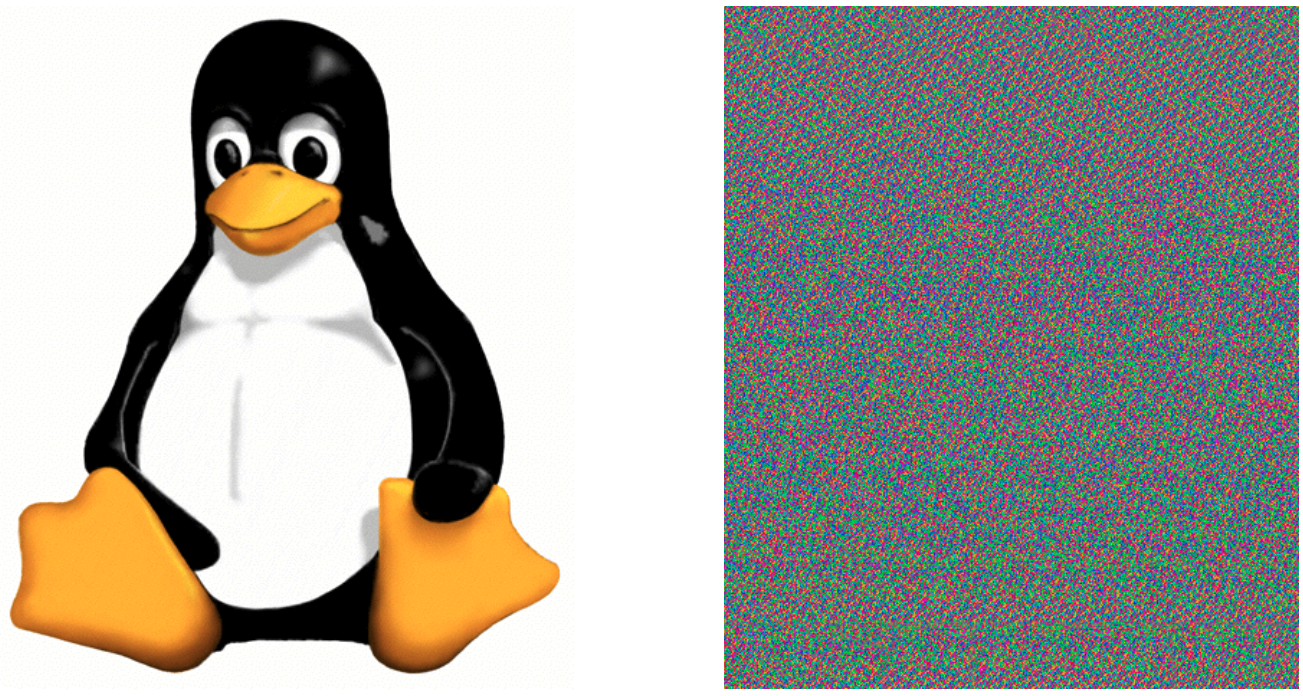
\includegraphics[width=0.7\textwidth]{Figure/CBC_Linux.png}
  \caption{Encrypted Image by CBC Mode}
\end{figure}
\end{minipage}

\subsection{Counter (CTR) Mode}
\begin{minipage}{0.5\textwidth}
For CTR mode, it supports parallel encryption and decryption, with provable security. This mode also selects a random IV (or nonce), and then the counter value for each block is incremented. \\[3pt]
Note that CTR decryption uses the block cipher's encryption function, not the decryption function.\\[3pt]
Both CTR and CBC achieve IND-CPA security if there is no reuse of the IV. Also, both modes require roughly the same amount of computation. However, CBC is parallelizable only for decryption, while CTR is parallelizable for both encryption and decryption.
\end{minipage}
\begin{minipage}{0.5\textwidth}
\begin{figure}[H]
  \centering
  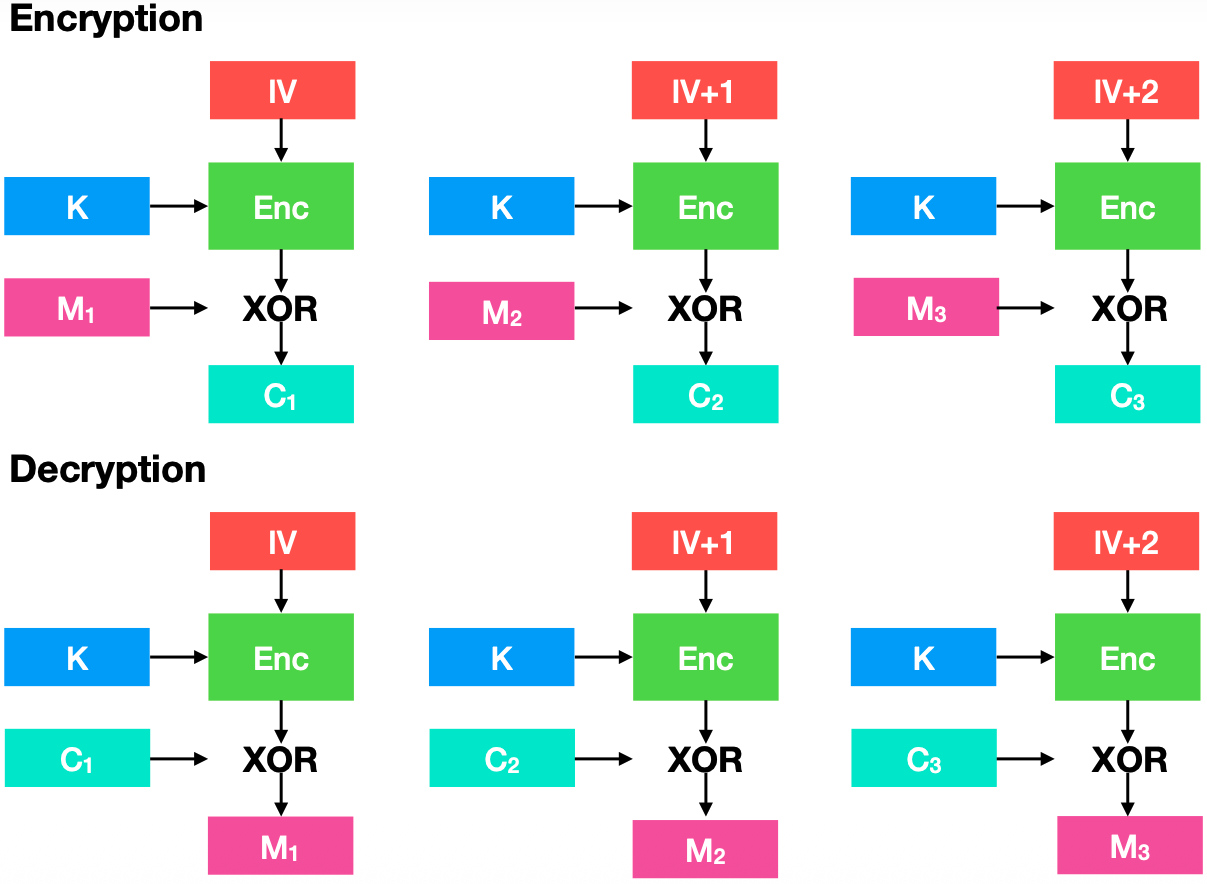
\includegraphics[width=0.7\textwidth]{Figure/CTR.png}
  \caption{CTR Mode}
\end{figure}
\end{minipage}

\subsection{Stream Ciphers}
\begin{minipage}{0.6\textwidth}
Block ciphers are fixed-size, stateless, and require modes to securely process longer messages. However, a stream cipher keeps state from previous messages and generates a one-time pseudo-random keystream \(K\).\\[3pt]
For a Pseudo-Random Number Generator (PRNG), given a seed, it outputs a sequence of seemingly random numbers and arbitrarily many random bits, while maintaining internal state. However, it cannot be truly random; instead, a cryptographically strong PRNG appears truly random to an attacker, since they cannot distinguish its output from a truly random sequence.
\end{minipage}
\begin{minipage}{0.38\textwidth}
\begin{figure}[H]
  \centering
  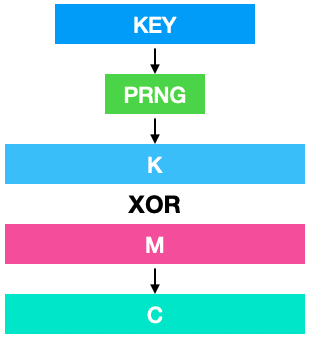
\includegraphics[width=0.6\textwidth]{Figure/StreamCiphers.png}
  \caption{Stream Ciphers}
\end{figure}
\end{minipage}

Thus, the key is used together with a state. Using a PRNG, we generate a keystream \(K\) that is used to encrypt the message. After choosing a random IV (initial state), we have
\[
  E(M, K) = \text{PRNG}(K, IV) \oplus M,
\]
and
\[
  D(C, K) = \text{PRNG}(K, IV) \oplus C.
\]

This is similar to the OTP, and it can produce any number of pseudo-random bits. It can also encrypt multiple messages.

\begin{remark}
  Block ciphers are stateless, meaning each encryption is independent and does not depend on previous inputs, so modes are needed to securely handle long messages. In contrast, stream ciphers maintain internal state and generate a pseudo-random keystream sequentially.
\end{remark}

After confidentiality, we also need to defend against active attacks.

\subsection{Integrity and Authentication}
Confidentiality alone is insufficient against active attacks. For an active attacker, they can inject new messages (ciphertexts), replay previous ciphertexts, and cause messages to be reordered or discarded. Therefore, for a message, we need to prove that it is not altered and is indeed sent from the sender. The approach to provide integrity is to use cryptographically strong hash functions.

There are properties that need to be satisfied:

1. One-way (pre-image resistance): ensure that given \(y\), it is difficult to find \(x\) such that \(\text{Hash}(x) = y\).

2. Collision resistance: ensure it is difficult to find \(x\) and \(x'\) such that \(\text{Hash}(x) = \text{Hash}(x')\).

3. Second pre-image resistance: ensure that given \(x\), it is difficult to find \(x'\) such that \(\text{Hash}(x) = \text{Hash}(x')\).

For example, SHA-256 and SHA-384 are two variants of the SHA-2 hash algorithm, returning 256-bit or 384-bit hashes. However, they are vulnerable to length-extension attacks. For example, suppose \(S\) is a secret, and the attacker knows \(\text{len}(S)\) and \(\text{Hash}(S)\). Then they can compute \(\text{Hash}(S \,\|\, M)\) for some \(M\), as the internal state can be derived from \(\text{Hash}(S)\) and \(\text{len}(S)\).

Since cryptographically strong hash functions alone are not sufficient for authentication (because attackers can also compute valid hash values), we introduce the Message Authentication Code (MAC).

\subsection{Message Authentication Code (MAC)}
This provides message integrity and authentication. It does not provide confidentiality and requires a shared secret key \(K\); the message itself can be in plaintext. 

For example, sender \(A\) computes \(T = \text{MAC}(M, K)\), then sends \(\{M, T\}\). Receiver \(B\) receives \(\{M', T'\}\), computes \(T'' = \text{MAC}(M', K)\), and compares \(T'\) with \(T''\).

Here, integrity is provided if the attacker cannot find \(M^*\) and \(T^*\) such that \(T^* = \text{MAC}(M^*, K)\), or find \(M^*\) such that \(T = \text{MAC}(M^*, K)\). This requires a combination of a strong hash function and a shared secret key.

\subsection{Hash-MAC (HMAC)}
To build a secure MAC, we consider the following components:

1. \(H\), which is a cryptographically strong hash function

2. \(\text{pad}_i, \text{pad}_o\), which are publicly known strings

3. \(K\), a secret key

Then we have
\[
  \text{HMAC}(M, K) = H\big((K \oplus \text{pad}_o) \,\|\, H((K \oplus \text{pad}_i) \,\|\, M)\big)
\]
which is believed to be secure even if \(H\) has certain weaknesses.

MACs in general do not provide any guarantee on confidentiality of the message, so it is recommended to compute the MAC using a secret key and apply it properly with encryption. For example, consider \(K_E\) as the encryption key and \(K_I\) as the MAC key:

1. SSL (MAC-then-Encrypt): \(C = E(M \,\|\, \text{MAC}(M, K_I), K_E)\)

2. SSH (Encrypt-and-MAC): \(C = E(M, K_E) \,\|\, \text{MAC}(M, K_I)\)

3. IPsec (Encrypt-then-MAC): \(C = E(M, K_E) \,\|\, \text{MAC}(E(M, K_E), K_I)\)

In summary, symmetric cryptography provides strong confidentiality but weak integrity and authenticity. Therefore, we introduce asymmetric cryptography.